\documentclass[11pt]{article}
\usepackage{geometry}                % See geometry.pdf to learn the layout options. There are lots.
\geometry{a4paper}                   % ... or a4paper or a5paper or ... 
%\geometry{landscape}                % Activate for for rotated page geometry
%\usepackage[parfill]{parskip}    % Activate to begin paragraphs with an empty line rather than an indent
\usepackage{graphicx}
\usepackage{amssymb}
\usepackage{amsmath}
\usepackage{lipsum}
\usepackage{authblk}
%\usepackage{amsaddr}
\usepackage{epstopdf}
\usepackage{booktabs}
\usepackage{bbold}
\usepackage{bm}
\usepackage{xcolor}
\usepackage{fancyhdr}
\usepackage[yyyymmdd,hhmmss]{datetime}
\pagestyle{fancy}
\rfoot{Compiled on \today\ at \currenttime}
\cfoot{}
\lfoot{Page \thepage}
\RequirePackage[colorinlistoftodos,prependcaption,textsize=tiny]{todonotes} % look for '\todo'
\definecolor{darkred}{rgb}{0.4,0.0,0.0}
\definecolor{darkgreen}{rgb}{0.0,0.4,0.0}
\definecolor{darkblue}{rgb}{0.0,0.0,0.4}
\usepackage[bookmarks,linktocpage,colorlinks,
    linkcolor = darkred,
    urlcolor  = darkblue,
    citecolor = darkgreen]{hyperref}

%\DeclareGraphicsRule{.tif}{png}{.png}{`convert #1 `dirname #1`/`basename #1 .tif`.png}

\renewcommand{\headrulewidth}{0pt}
\fancyhead[L]{
%\includegraphics[width=4cm]{/Users/tomluu/Research/talks/fzjTemplate/uniBonn_logo.jpg}
}
\fancyhead[R]{

\includegraphics[width=4cm]{figs/fzj_logo.jpg}
}
\pagestyle{plain}

\title{Understanding finite-volume corrections to spherical L\"uscher}
\author[1,2]{Thomas Luu}
\affil[1]{Institute for Advanced Simulation 4\\
Forschungszentrum J\"ulich, Germany}
\affil[2]{Rheinische Friedrich-Williams-Universit\"at Bonn, Germany}

%\email{t.luu@fz-juelich.de}
\date{}                                           % Activate to display a given date or no date


\begin{document}
\maketitle
\begin{center}
email: \href{mailto:t.luu@fz-juelich.de}{t.luu@fz-juelich.de}
\end{center}
\abstract{
Ok, I show that the L\"uscher dispersion formula is equivalent to solving the Schr\"odinger equation, and derive the linear and quadratic behavior found when using the spherical L\"uscher formula with contact interaction.
}

\thispagestyle{fancy}

\clearpage{}
%\tableofcontents
%\newpage

\section{Dispersion L\"uscher (with contact interaction) is really the Schr\"odinger equation in disguise}

Ok, I assume I live in a cubic box of side length $L$ and space is discretized with lattice spacing $\epsilon$ corresponding to $N$ sites per side. Also, I only have a contact interaction for the time being,
\begin{equation}
\langle \bm n|\hat V|\bm m\rangle = C_0(\Lambda)\ .%\Theta\left(|\bm n|-\frac{\Lambda L}{2\pi}\right)\Theta\left(|\bm m|-\frac{\Lambda L}{2\pi}\right)\ .
\end{equation}
For now I don't assume anything about $\Lambda$, i.e. I treat it as just some parameter.  The states $|\bm n\rangle$ are eigenvectors of the non-interacting Hamiltonian\footnote{I assume an $n_{step}=\infty$ dispersion, but the results of this section also hold for finite $n_{step}$.},
\begin{equation}
\hat H_0|\bm n\rangle = \frac{4\pi^2}{mL^2}\bm n^2|\bm n\rangle\ .
\end{equation}
The Schr\"odinger equation with this interaction is
\begin{equation}\label{eqn:schroedinger}
\left(\hat H_0+\hat V\right)|\psi\rangle = E|\psi\rangle\ ,
\end{equation}
where $|\psi\rangle$ is an eigenstate and $E$ is its corresponding eigenvalue.  I now put eq.~\eqref{eqn:schroedinger} into its integral form,
\begin{equation}\label{eqn:integral form 1}
|\psi\rangle = \frac{1}{E-\hat H_0}\hat V|\psi\rangle\ ,
\end{equation}
and act with $\langle \bm n|$ from the left,
\begin{equation}\label{eqn:integral form 2}
\langle \bm n|\psi\rangle = \frac{1}{E-\frac{4\pi^2}{mL^2}\bm n^2}\langle \bm n|\hat V|\psi\rangle\ .
\end{equation}
Note that the closure relation in a discretized box is
\begin{equation}\label{eqn:closure}
\hat 1=\frac{1}{L^3}\sum_{\bm n \in (-N/2,N/2]^3}|\bm n\rangle \langle \bm n|=\frac{1}{L^3}\sum_{\bm n \in \mathrm{B.Z.}}|\bm n\rangle \langle \bm n|\ .
\end{equation}
I simplify notation by replacing $\bm n \in (-N/2,N/2]^3$ with $\bm n \in\mathrm{B.Z.}$ where B.Z. stands for 1st Brillouin Zone. So now I insert a complete set of states into eq.~\eqref{eqn:integral form 2},
\begin{multline}\label{eqn:integral form 3}
\langle \bm n|\psi\rangle =\frac{1}{L^3} \sum_{\bm m\in\mathrm{B.Z.}}\frac{1}{E-\frac{4\pi^2}{mL^2}\bm n^2}\langle \bm n|\hat V|\bm m\rangle \langle \bm m|\psi\rangle\\
=\frac{1}{L^3} \sum_{\bm m\in\mathrm{B.Z.}}\frac{C_0(\Lambda)}{E-\frac{4\pi^2}{mL^2}\bm n^2} \langle \bm m|\psi\rangle\ .
\end{multline}
I now sum over all vectors $\bm n$ in the first B.Z.,
\begin{multline}
\sum_{\bm n\in \mathrm{B.Z.}}\langle \bm n|\psi\rangle =\frac{1}{L^3} \sum_{\bm n,\bm m\in\mathrm{B.Z.}}\frac{C_0(\Lambda)}{E-\frac{4\pi^2}{mL^2}\bm n^2} \langle \bm m|\psi\rangle\\
=\sum_{\bm m\in \mathrm{B.Z.}}\langle \bm m|\psi\rangle\frac{1}{L^3} \sum_{\bm n\in\mathrm{B.Z.}}\frac{C_0(\Lambda)}{E-\frac{4\pi^2}{mL^2}\bm n^2}\ .
\end{multline}
I can now move everything to the LHS (and rename some dummy variables),
\begin{equation}
\sum_{\bm m\in \mathrm{B.Z.}}\langle \bm m|\psi\rangle\left(1-\frac{1}{L^3} \sum_{\bm n\in\mathrm{B.Z.}}\frac{C_0(\Lambda)}{E-\frac{4\pi^2}{mL^2}\bm n^2}\right)=0\ .
\end{equation}
So this expression holds if\footnote{The expression also holds if
\begin{displaymath}
\sum_{\bm m\in \mathrm{B.Z.}}\langle \bm m|\psi\rangle=0\ ,
\end{displaymath}
but I believe that such a condition cannot be true in general.  Can someone prove this?}
\begin{align}
1-&\frac{1}{L^3} \sum_{\bm n\in\mathrm{B.Z.}}\frac{C_0(\Lambda)}{E-\frac{4\pi^2}{mL^2}\bm n^2}=0\nonumber\\
\implies& \frac{-1}{C_0(\Lambda)}=\frac{1}{L^3}\sum_{\bm n\in\mathrm{B.Z.}}\frac{1}{\frac{4\pi^2}{mL^2}\bm n^2-E}\ .\label{eqn:almost there}
\end{align}
I manipulate eq.~\eqref{eqn:almost there} just a little to make it look more familiar,
\begin{equation}
 \frac{-4\pi/m}{C_0(\Lambda)}=\frac{1}{\pi L}\sum_{\bm n\in\mathrm{B.Z.}}\frac{1}{\bm n^2-x}\ .\label{eqn:really almost there}
 \end{equation}
 where 
 \begin{equation}
 x\equiv \frac{mEL^2}{4\pi^2}\ .
 \end{equation}
\emph{Given some coefficient $C_0(\Lambda)$ for the delta interaction, the (dimensionless) eigenvalues $x$ that satisfy Schr\"odinger's equation~\eqref{eqn:schroedinger} (with this interaction) will also satisfy the self-consistent equation~\eqref{eqn:really almost there}.  This is because eq.~\eqref{eqn:really almost there} and eq.~\eqref{eqn:schroedinger} are really the same thing.  This holds for \emph{any} $C_0(\Lambda)$.}

Of course we tune $C_0(\Lambda)$ to reproduce some observable in the infinite-volume limit, which in this case is the scattering length $a_0$,
\begin{equation}\label{eqn:C0(lambda)}
C_0(\Lambda)=\frac{-4\pi/m}{\frac{-1}{a_0}+\mathcal{L}^\square_3\frac{\Lambda}{4\pi^2}}\ ,
\end{equation}
where $\mathcal{L}^\square_3=15.348248444887464047104634$. I now identify the cutoff $\Lambda$ with the lattice spacing $\epsilon$,
\begin{equation}
\frac{1}{\epsilon}=\frac{\Lambda}{2\pi}=\frac{N}{L}\ ,
\end{equation}
allowing me to trade $\Lambda$ for the ratio $N/L$ in eq.~\eqref{eqn:C0(lambda)},
\begin{equation}\label{eqn:C0(N)}
C_0(N/L)=\frac{-4\pi/m}{\frac{-1}{a_0}+\mathcal{L}^\square_3\frac{N}{2\pi L}}\ .
\end{equation}
Plugging this expression into eq.~\eqref{eqn:really almost there} gives the desired result,
\begin{equation}\label{eqn:finally there}
\frac{-1}{a_0}=\frac{1}{\pi L}\left(\sum_{\bm n\in\mathrm{B.Z.}}\frac{1}{\bm n^2-x}-\mathcal{L}^\square_3\frac{N}{2}\right)\quad\quad\left(=\frac{1}{\pi L}S^{\square N}_3(x)\right)\ .
\end{equation}
I stress again:  for the coefficient of the delta function interaction given by eq.~\eqref{eqn:C0(N)}, the eigenvalues $x$ of the Schr\"odinger equation with this interaction will exactly satisfy the relation in eq.~\eqref{eqn:finally there}, which is our dispersion L\"uscher formula.  

\section{Corrections to the spherical L\"uscher formula}
What happens when one takes values of $x$, calculated with a delta function interaction in a box of side length $L$ with $N$ points per side, and plugs it instead into the spherical L\"uscher formula\footnote{Here I must constrain myself to an $n_{step}=\infty$ analysis.  Maybe there's a way to do this with finite $n_{step}$?},
\begin{equation}\label{eqn:spherical luscher}
\frac{1}{\pi L}S^\bigcirc_3(x)=\lim_{\eta \to\infty}\frac{1}{\pi L}\left(\sum_{\bm n}^{|\bm n|<\eta / 2} \frac{1}{\bm n^{2}-x}-\mathcal{L}^\bigcirc_3\frac{\eta}{2}\right)\ \ ?
\end{equation}
Here $\mathcal{L}^{\bigcirc}_3\equiv 4\pi$.  Let's find out\ldots

I can separate out the dispersion L\"uscher formula from eq.~\eqref{eqn:spherical luscher} by adding and subtracting it,
\begin{multline}
\frac{1}{\pi L}S^\bigcirc_3(x)=\frac{1}{\pi L}\left(S^{\square N}_3+\left(S^\bigcirc_3(x)-S^{\square N}_3\right)\right)=\frac{-1}{a_0}+\frac{1}{\pi L}\left(S^\bigcirc_3(x)-S^{\square N}_3\right)\\
=\frac{-1}{a_0}+\lim_{\eta \to\infty}\frac{1}{\pi L}\left(\sum_{\bm n\notin \mathrm{B.Z.}}^{|\bm n|<\eta / 2} \frac{1}{\bm n^{2}-x}-\mathcal{L}^\bigcirc_3\frac{\eta}{2}+\mathcal{L}^\square_3\frac{N}{2}\right)
\end{multline}
Since $\bm n$ is now restricted to be \emph{outside} the B.Z., I can assume that $\bm n^2\gg x$ which allows me to Taylor expand under the summation,
\begin{align}
S^\bigcirc_3(x)=&\frac{-\pi L}{a_0}\label{eqn:observable}\\
&+\mathcal{L}^\square_3\frac{N}{2}+\lim_{\eta \to\infty}\left(\sum_{\bm n\notin \mathrm{B.Z.}}^{|\bm n|<\eta / 2} \frac{1}{\bm n^{2}}-\mathcal{L}^\bigcirc_3\frac{\eta}{2}\right)\label{eqn:constant}\\
&+x\lim_{\eta \to\infty}\sum_{\bm n\notin \mathrm{B.Z.}}^{|\bm n|<\eta / 2} \frac{1}{\bm n^{4}}\label{eqn:range}\\
&+x^2\lim_{\eta \to\infty}\sum_{\bm n\notin \mathrm{B.Z.}}^{|\bm n|<\eta / 2} \frac{1}{\bm n^{6}}\label{eqn:shape}\\
&\vdots
\end{align}
All terms above involving summations have an implicit dependence on $N$ due to the fact that the vector $\bm n$ is excluded from the B.Z.  The summations in eqs.~\eqref{eqn:range} and~\eqref{eqn:shape} converge, albeit slowly.  The expression in eq.~\eqref{eqn:constant}  requires acceleration, but also special care because the summation diverges linearly.  

To evaluate these sums, I first replace all summations by the following,
\begin{equation}
\sum_{\bm n\notin \mathrm{B.Z.}}^{|\bm n|<\eta / 2} \to
\left(\sum_{|\bm n|\ne 0}^{|\bm n|<\eta / 2} -\sum_{\bm n \in \mathrm{B.Z.}\ \&\ 
 |\bm n|\ne 0}\right)
\end{equation}
This is an equivalent replacement.  I now define
\begin{align}
\mathcal{I}_1&\equiv \lim_{\eta \to\infty}\left(\sum_{|\bm n|\ne 0}^{|\bm n|<\eta / 2} \frac{1}{\bm n^{2}}-\mathcal{L}^\bigcirc_3\frac{\eta}{2}\right)&;  &\quad
\mathcal{J}_1^N=\sum_{\bm n \in \mathrm{B.Z.}\ \&\ 
 |\bm n|\ne 0} \frac{1}{\bm n^{2}}-\mathcal{L}^\square_3\frac{N}{2}\label{eqn:1}\\
\mathcal{I}_{\alpha>1}&\equiv\lim_{\eta \to\infty}\sum_{|\bm n|\ne 0}^{|\bm n|<\eta / 2} \frac{1}{\left(\bm n^{2}\right)^\alpha}&;&\quad
\mathcal{J}_{\alpha>1}^N=\sum_{\bm n \in \mathrm{B.Z.}\ \&\ 
 |\bm n|\ne 0} \frac{1}{\left(\bm n^{2}\right)^\alpha}\label{eqn:alpha}
\end{align}
 The $\mathcal{I}_\alpha$ terms (particularly $\mathcal{I}_1$) require acceleration techniques for their numerical determination.  \autoref{tab:I coefficients} provides the numerical values of these coefficients.
\begin{table}
\caption{The coefficients $\mathcal{I}_\alpha$ obtained via acceleration techniques.  Results are good to the number of decimal points shown. \label{tab:I coefficients}}
\center
\begin{tabular}{c|c|c}
$\mathcal{I}_1$ & $\mathcal{I}_2$ &$\mathcal{I}_3$\\
\hline
-8.91363291758515127269 & 16.532315959761669643893 & 8.4019239748275399931461\\
\end{tabular}
\end{table}
All the $N$ dependence is now in the $\mathcal{J}_\alpha^N$ coefficients which can be numerically calculated directly to arbitrary precision.  In \autoref{tab:J coefficients} I provide numerical values of $\mathcal{J}_\alpha^N$ for select values of $N$.

With the definitions in eqs.~\eqref{eqn:1} and~\eqref{eqn:alpha} the spherical L\"uscher formula evaluated using $x$ (from a discretized box calculation) can be expressed as
\begin{equation}
S^\bigcirc_3(x)=\frac{-\pi L}{a_0}+\left(\mathcal{I}_1-\mathcal{J}_1^N\right)+x\left(\mathcal{I}_2-\mathcal{J}_2^N\right)+x^2\left(\mathcal{I}_3-\mathcal{J}_3^N\right)+\ldots
\end{equation}
Note that even if $|a_0|\to\infty$, there is still a constant shift due to $\left(\mathcal{I}_1-\mathcal{J}_1^N\right)$.   
\begin{table}
\caption{The coefficients $\mathcal{J}_\alpha^N$ for select values of $N$.  Results are good to the number of decimal points shown. \label{tab:J coefficients}}
\center
\begin{tabular}{c||c|c|c}
$N$ & $\mathcal{J}_1^N$ & $\mathcal{J}_2^N$ &$\mathcal{J}_3^N$ \\
\hline
10 & -9.25986138777860 & 14.4234798298591 & 8.38095669349515\\
20 & -9.08747321556999 & 15.4853107114944 & 8.39938622894022\\
40 & -9.00064439734243 & 16.0097506821086 & 8.40160941170844\\
50 & -8.98325088166483 & 16.1143539592680 & 8.40176308245080\\
80 & -8.95715009201217 & 16.2711508329433 & 8.40188473787034\\
100 & -8.94844775523651 & 16.3233951468942 & 8.40190389063797
\end{tabular}
\end{table}
These numbers allow us to determine the coefficients of the $x$ and $x^2$ terms.  For example, with $N=100$, I find
\begin{multline}
S^\bigcirc_3(x)=\frac{-\pi L}{a_0}\\
+0.03481483765136+0.2089208128674 x+0.00002008418957 x^2+\ldots
\end{multline}
\autoref{tab:slopes} gives the coefficients of the $x$ and $x^2$ terms for other values of $N$.
\begin{table}
\caption{Coefficients of $x$ and $x^2$ terms as a function of $N$\label{tab:slopes}}
\center
\begin{tabular}{c|c}
$N$ & $S^\bigcirc_3(x)+\frac{\pi L}{a_0}$ \\
\hline
10 & $0.34622847019345+2.1088361299026 x+0.02096728133239 x^2$\\
20 & $0.17384029798483+1.0470052482673 x+0.00253774588732 x^2$\\
40 & $0.08701147975728+0.5225652776531 x+0.00031456311910 x^2$\\
50 & $0.06961796407968+0.4179620004936 x+0.00016089237674 x^2$\\
80 & $0.04351717442702+0.2611651268184 x+0.00003923695720 x^2$\\
100 &$0.03481483765136+0.2089208128674 x+0.00002008418957 x^2$
\end{tabular}
\end{table}

In \autoref{fig:S3 figure} I show the resulting function for $S^\bigcirc_3(x)/\pi$ for $N=10,20,40,50,80,100$.  Here I assume that $|a_0|=\infty$\footnote{When comparing with fig.4 of our manuscript, the scales look familiar, but I do not understand how the y-axis is defined in fig.4.}.
\begin{figure}
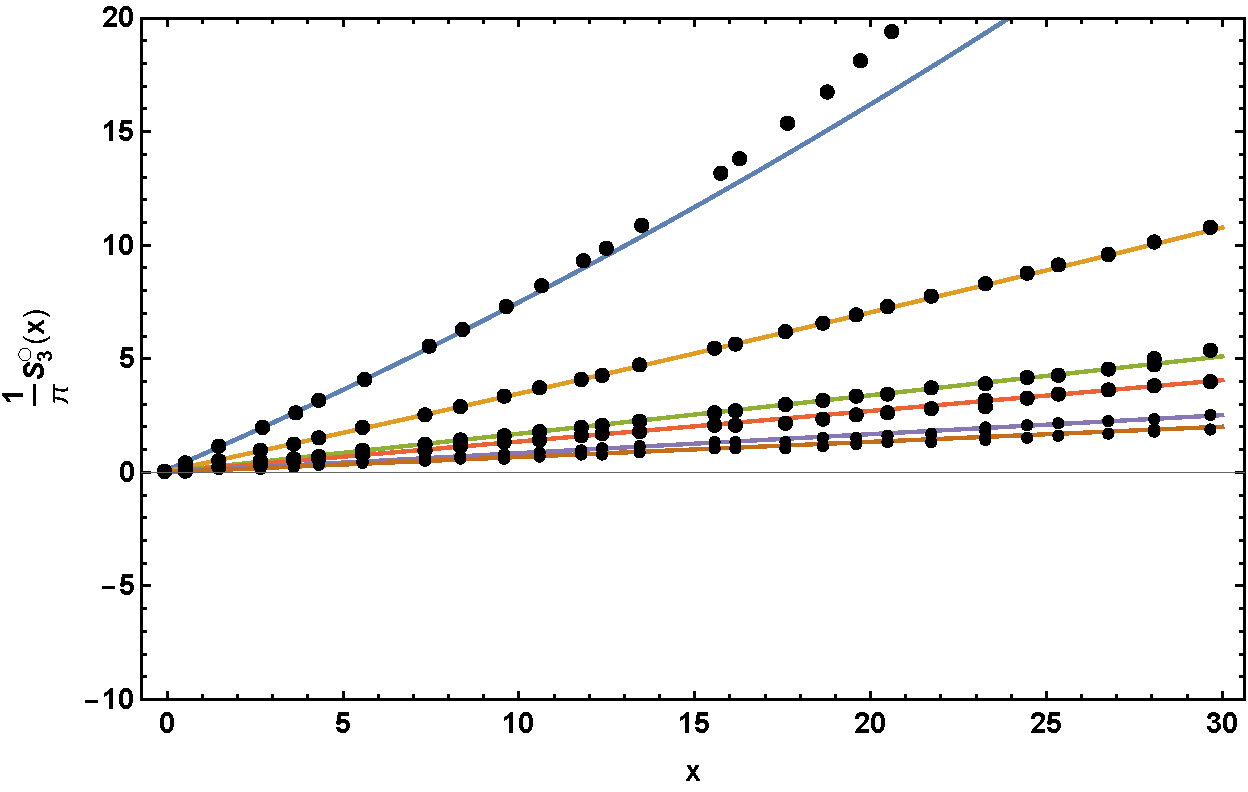
\includegraphics[width=\textwidth]{figs/S3_figure.pdf}
\caption{Plot of spherical L\"uscher as a function of $x$ for $N=10,20,40,50,80,100$.  \label{fig:S3 figure}}
\end{figure}
I also provide numerical calculations (black dots) that were determined in the following manner:
\begin{itemize}
\item I set $|a_0|\to\infty$
\item Given some $N$, I solve for the zeros of eq.~\eqref{eqn:finally there}.  This provides me with a list of $x$ values corresponding to the eigenvalues of the Schr\"odinger equation
\item I feed these values through a numerical implementation of the spherical L\"uscher formula, obtaining the black points shown in \autoref{fig:S3 figure}
\end{itemize}
The level of agreement between the black points and the curves suggest that I'm doing something right.  We can now improve on the spherical L\"uscher result by subtracting off this dependence.

%\newpage
%\appendix

%\clearpage
%\bibliography{references}

\end{document}  
